\chapter{Results}
\label{Results}

We will first present our results pertaining to warning adherence by comparing user compliance for the control (Firefox default) warnings against our tiered messages. We will then delve into user understanding, making similar comparisons and examining reaction times and user ratings of warning severity.


\section{Warning Adherence}
\label{Warning Adherence}
\subsection{Control Warning Message Adherence}
The mean control warning message adherence rates for both phases of the study are summarized below in table \ref{tab:Adherence-Control}. For context, the number of participants for each value is also included. 

{\renewcommand{\arraystretch}{1.2}
\begin{table}[!htb]
	\small
	\centering
	\begin{tabularx}{0.85\textwidth}{|l|X|X|}
		\hline			
		\textbf{Warning Type} & \multicolumn{2}{|X|}{\textbf{Adherence Rate}}\\
		\cline{2-3}
		& \textbf{Phase 1} & \textbf{Phase 2}\\
		\hline
		SSL & 50\% (1/2) & 60\% (12/20)\\
		\hline
		Malware & 0\% (0/1) & 90\% (18/20)\\
		\hline
		Phishing & 100\% (1/1) & 80\% (16/20)\\
		\hline
		Unwanted Software & 100\% (1/1) & 85\% (17/20)\\
		\hline
	\end{tabularx}
	\caption{Control warning message adherence rates}
	\label{tab:Adherence-Control}
\end{table}}

With the exception of the malware warning in phase 1, the SSL warning had the lowest adherence rate. This is consistent with the findings of Felt et al. \cite{felt2015improving}.

\subsection{Tiered Warning Message Adherence}
The mean tiered warning message adherence rates for both phases of the study are summarized below in table \ref{tab:Adherence-Tiered}. For context, the number of participants for each value is also included.

{\renewcommand{\arraystretch}{1.2}
\begin{table}[!htb]
	\small
	\centering
	\begin{tabularx}{0.85\textwidth}{|l|l|X|X|}
		\hline
		\multicolumn{2}{|l|}{\textbf{Warning}} & \multicolumn{2}{|X|}{\textbf{Adherence Rate}}\\
		\hline
		\textbf{Type} & \textbf{Severity} & \textbf{Phase 1} & \textbf{Phase 2}\\
		\specialrule{.1em}{.0em}{.0em} 
		SSL & Low & 0\% (0/2) & 35\% (7/20)\\
		\cline{2-4}
		& Medium & 0\% (0/2) & 55\% (11/20)\\
		\cline{2-4}
		& High & 0\% (0/2) & 80\% (16/20)\\
		\specialrule{.1em}{.0em}{.0em} 
		Malware & Low & 100\% (1/1) & 45\% (9/20)\\
		\cline{2-4}
		& Medium & 0\% (0/1) & 65\% (13/20)\\
		\cline{2-4}
		& High & 100\% (1/1) & 100\% (20/20)\\
		\specialrule{.1em}{.0em}{.0em} 
		Phishing & Low & 100\% (1/1) & 45\% (9/20)\\
		\cline{2-4}
		& Medium & 100\% (1/1) & 65\% (13/20)\\
		\cline{2-4}
		& High & 100\% (1/1) & 95\% (19/20)\\
		\specialrule{.1em}{.0em}{.0em} 
		Unwanted S/W & Low & 0\% (0/1) & 45\% (9/20)\\
		\cline{2-4}
		& Medium & 0\% (0/1) & 65\% (13/20)\\
		\cline{2-4}
		& High & 0\% (0/1) & 75\% (15/20)\\
		\hline
	\end{tabularx}
	\caption{Tiered warning message adherence rates}
	\label{tab:Adherence-Tiered}
\end{table}}

In phase 1, all phishing and malware warnings (except for the medium severity malware warning) were adhered to every time. Every other type and severity of warning was ignored. In phase 2, adherence intuitively increases with severity for all message types (illustrated below in figure \ref{fig:Adherence-Tiered}).

\begin{figure}[!htb]
	\centering
	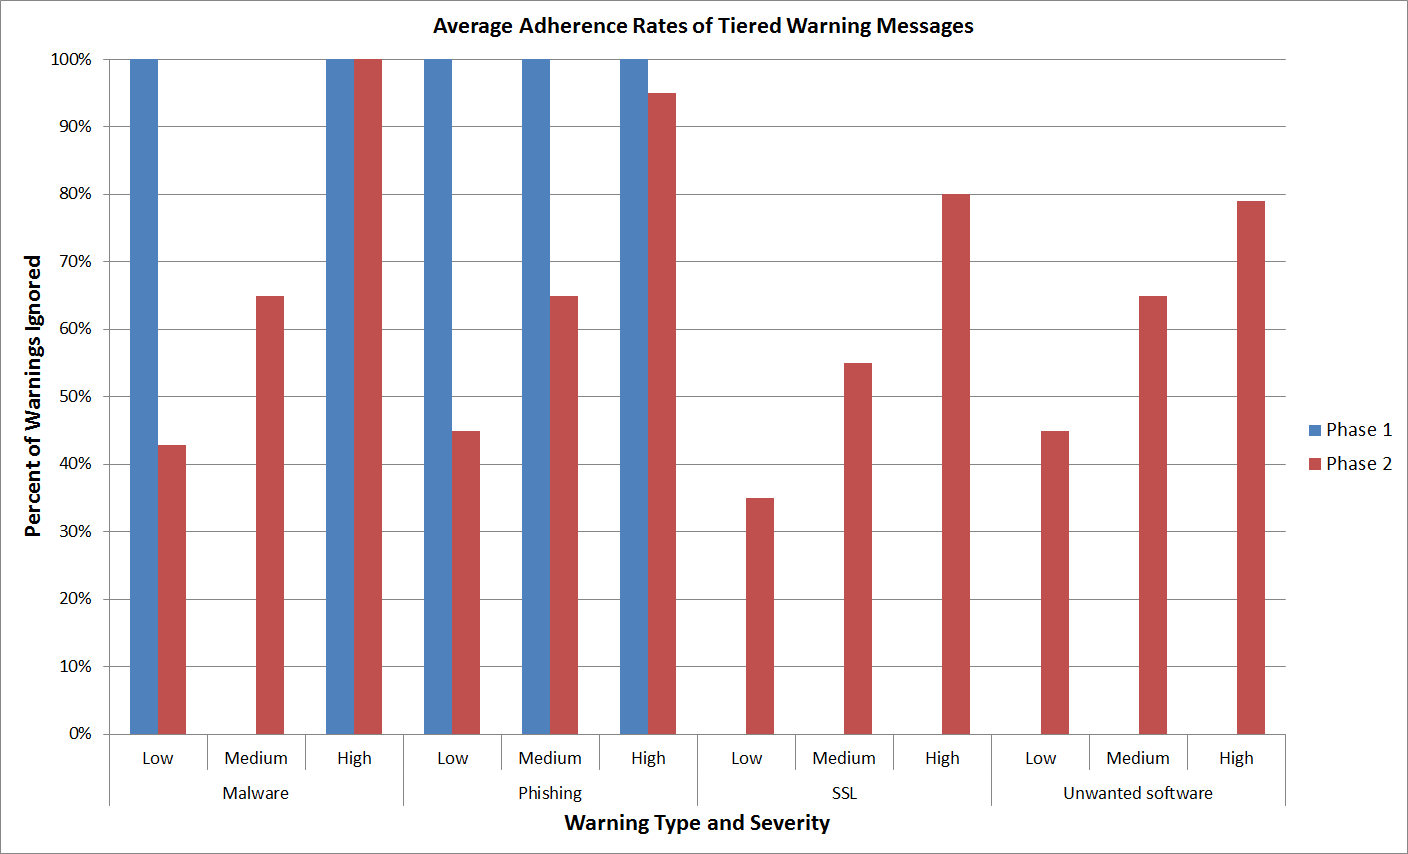
\includegraphics[width=\textwidth]{Figures/Adherence-Tiered}
	\decoRule
	\caption{Tiered warning message adherence rates}
	\label{fig:Adherence-Tiered}
\end{figure}

\subsection{Warning Message Adherence Analysis}
Six separate two-tailed t-tests were conducted. For each of the study phases, the mean adherence rate for the control warning messages was separately compared against the mean adherence rate for the low, medium, and high severity tiered messages.

In the first phase of the study, the mean adherence rate was always lower for the tiered messages than for the control ones. This difference was not found to be statistically significant.

In the second phase of the study, the mean adherence rates for the low and medium severity tiered warnings were lower than the control warnings (41.3\% and 62.5\%, respectively, versus 78.8\%). These differences in adherence rates were found to be statistically significant ($t(19) = 4.81, p = 0.0001$ in the the low severity versus control case and $t(19) = 2.94, p = 0.0084$ in the high severity versus control case).

The mean adherence rate in of the high severity tiered warnings in phase 2 was greater than that of the control warnings (88.8\% versus 78.8\%). This difference was found to be statistically significant ($t(19) = -2.37, p = 0.028$).

In summary, in phase 2, users were significantly more likely to adhere to our ``severe'' tiered messages and significantly less likely to adhere to our ``low'' and ``medium'' tiered messages, compared to the control messages.


\section{Reaction Time}
For each warning message presented in the study, our software measured the time that elapsed between when it was first shown and when participants made a decision (i.e., clicked either the ``ignore'' or ``go back'' button). For both the control and tiered messages, participants exhibited similar behaviour for decisions made within the first 20 seconds of being presented with a warning.

\subsection{Reaction Time for Control Warning Messages}
\begin{figure}[!htb]
	\centering
	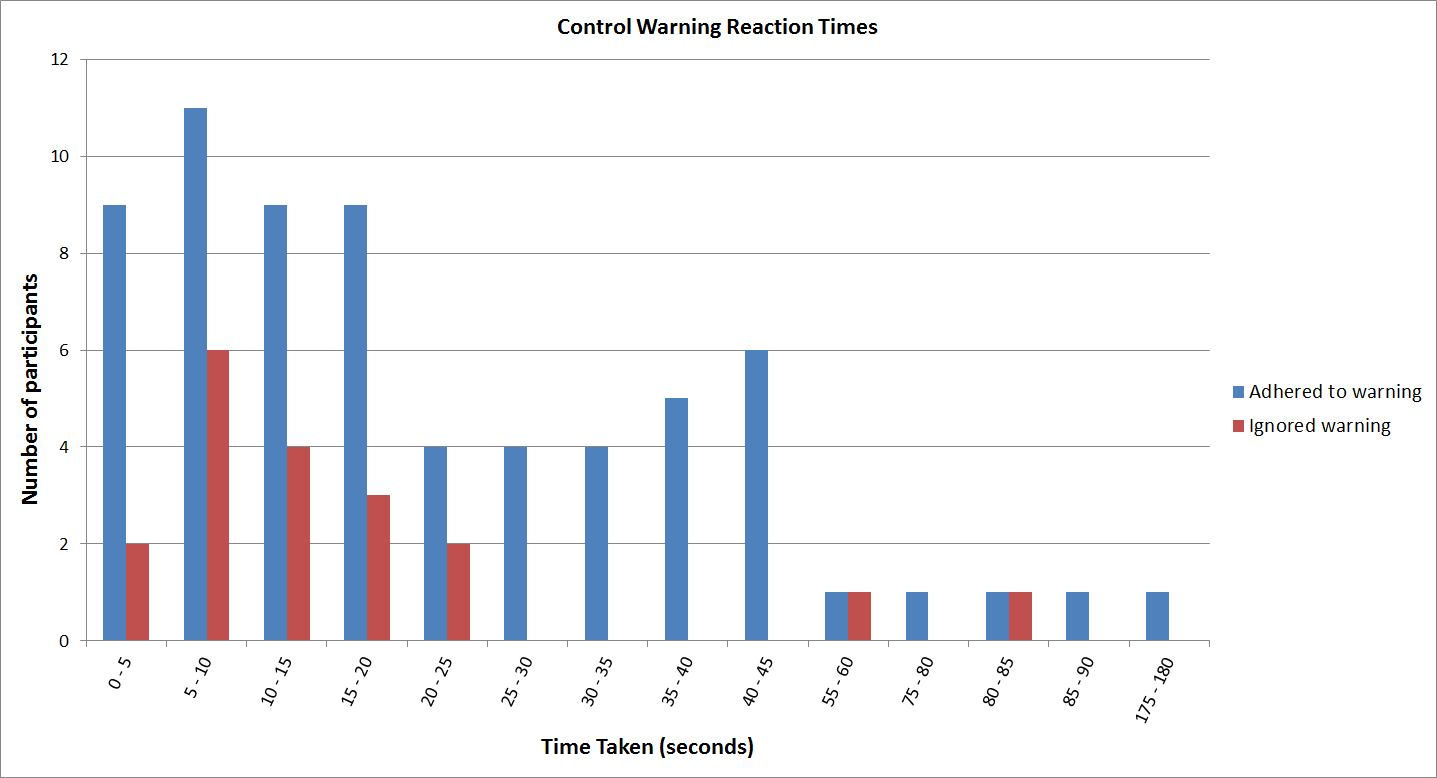
\includegraphics[width=\textwidth]{Figures/Time-Control}
	\decoRule
	\caption[Control warning decision times]{The amount of time taken by participants to make decisions regarding the control warning messages.}
	\label{fig:Time-Control}
\end{figure}
Most participants took between 5 and 10 seconds to make a decision after being faced with a control warning message (20\%). The rates of adherence and dismissal follow similar, bell curve-like distributions for relatively short times (below 20 seconds). For slightly longer times (between 20 and 45 seconds), adherence intuitively increases as the time spent observing the warning message increases. Additionally, dismissal in general does not occur as often beyond 20 seconds (only 12.5\% of the time). These results are illustrated in figure \ref{fig:Time-Control}.

\subsection{Reaction Time for Tiered Warning Messages}
These results are similar to those seen for the control warning messages. Again, most participants took between 5 and 10 seconds to make a decision (32.55\%). Unlike the control warnings, the majority of participants took less than 30 seconds to make a decision regarding the tiered messages (93.33\%). The rates of adherence and dismissal follow similar distributions: a steep increase before the 10 second mark and a decline afterwards. These results are illustrated in figure \ref{fig:Time-Tiered}.

\begin{figure}[!htb]
	\centering
	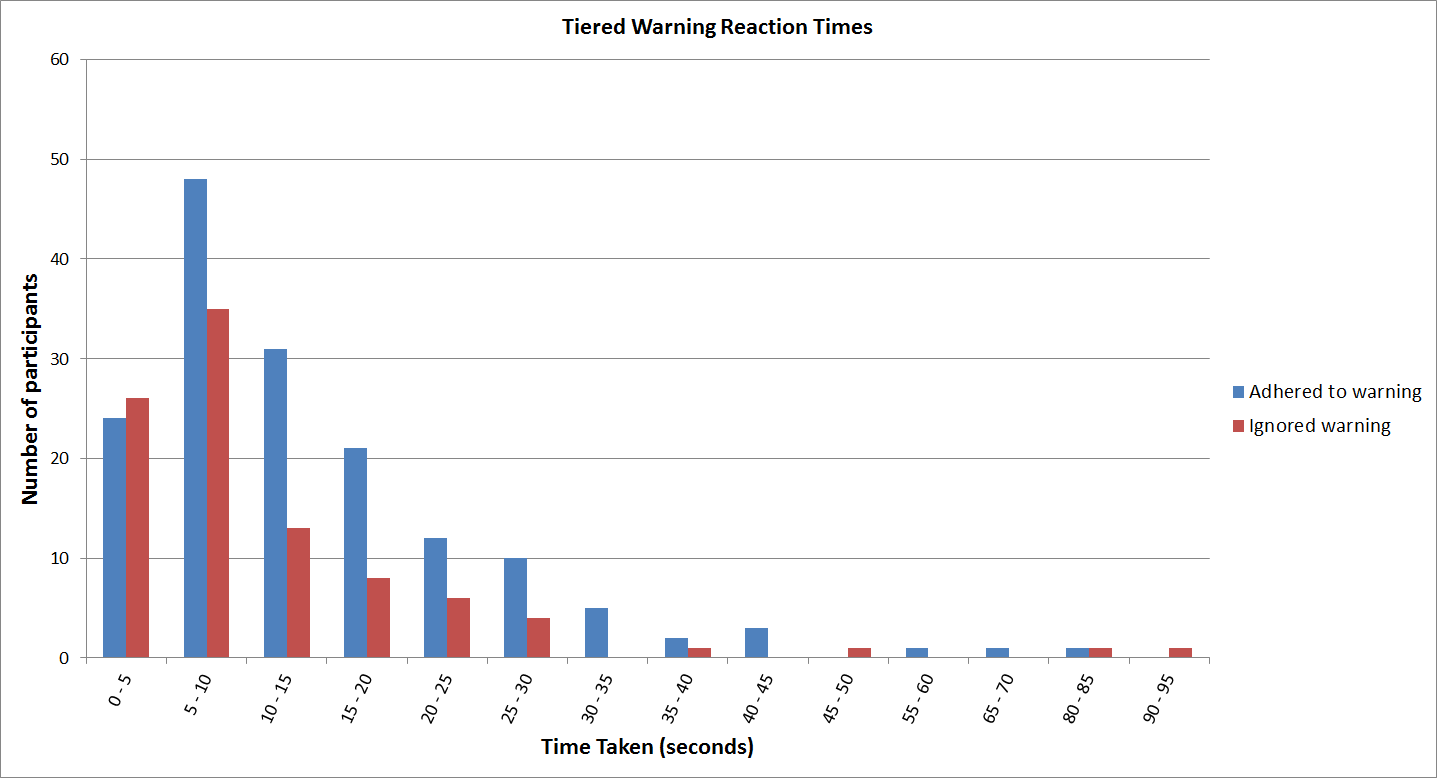
\includegraphics[width=\textwidth]{Figures/Time-Tiered}
	\decoRule
	\caption[Tiered warning decision times]{The amount of time taken by participants to make decisions regarding the tiered warning messages.}
	\label{fig:Time-Tiered}
\end{figure}

\subsection{Reaction Time Analysis}
The mean time taken to make a decision was compared between the control messages and the tiered messages in a two-tailed paired t-test. The average time was lower for the tiered messages than for the control messages (13.44 seconds versus 23.26 seconds, respectively) and the difference was found to be statistically significant ($t(19)=5.06, p=0.00007$).

This could mean that our tiered message express the warning content and severity more clearly to participants (making their decisions faster and easier), or alternately, that they come across as less important and are thereby more quickly dismissed. See section \ref{Discussion} for further discussion.


\section{Severity Rating}
For each warning message, participants were presented with an on-screen questionnaire after they chose to either adhere to or ignore it. The first question asked them to rate the message's severity on a 5-point Likert scale (with 0 being the least severe and 4 being the most severe). Consistent with the adherence rates in section \ref{Warning Adherence}, SSL ratings are generally rated the least severe.

\subsection{Control Warning Message Severity Ratings}
The average control warning message user severity ratings for both phases of the study are summarized below in table \ref{tab:Severity-Control}. For context, the number of participants for each value is also included. Participants generally chose higher ratings in phase 2, with the exception of the unwanted software warning.

{\renewcommand{\arraystretch}{1.2}
\begin{table}[!htb]
	\small
	\centering
	\begin{tabularx}{0.85\textwidth}{|l|X|X|}
		\hline			
		\textbf{Warning Type} & \multicolumn{2}{|X|}{\textbf{Severity Rating}}\\
		\cline{2-3}
		& \textbf{Phase 1} & \textbf{Phase 2}\\
		\hline
		SSL & 1.00 (2 participants) & 1.55 (20 participants)\\
		\hline
		Malware & 1.00 (1 participant) & 3.20 (20 participants)\\
		\hline
		Phishing & 2.00 (1 participant) & 3.00 (20 participants)\\
		\hline
		Unwanted Software & 4.00 (1 participant) & 3.05 (20 participants)\\
		\hline
	\end{tabularx}
	\caption{Control warning message severity ratings}
	\label{tab:Severity-Control}
\end{table}}

\subsection{Tiered Warning Message Severity Ratings}
The average tiered warning message user severity ratings for both phases of the study are summarized below in table \ref{tab:Severity-Tiered}. For context, the number of participants for each value is also included.

User severity ratings for low and medium tiered warnings were generally higher in the first phase of the study than the second. All high severity warnings were rated between 3 and 4 (between ``high'' and ``very high'' severity on our Likert scale) and all low severity ratings were rated between 0 and 2 (between ``very low'' and ``medium'' severity on our Likert scale). Additionally, the ratings in phase 2 of the study predictably increase with severity, similar to the adherence rates in section \ref{Warning Adherence} (illustrated below in figure \ref{fig:Severity-Tiered}).

{\renewcommand{\arraystretch}{1.2}
\begin{table}[!htb]
	\small
	\centering
	\begin{tabularx}{\textwidth}{|l|l|X|X|}
		\hline
		\multicolumn{2}{|l|}{\textbf{Warning}} & \multicolumn{2}{|X|}{\textbf{Severity Rating}}\\
		\hline
		\textbf{Type} & \textbf{Severity} & \textbf{Phase 1} & \textbf{Phase 2}\\
		\specialrule{.1em}{.0em}{.0em} 
		SSL & Low & 2.00 (2 participants) & 0.80 (20 participants)\\
		\cline{2-4}
		& Medium & 3.50 (2 participants) & 1.70 (20 participants)\\
		\cline{2-4}
		& High & 0.00 (2 participants) & 3.28 (20 participants)\\
		\specialrule{.1em}{.0em}{.0em} 
		Malware & Low & 2.00 (1 participant) & 1.19 (20 participants)\\
		\cline{2-4}
		& Medium & 2.00 (1 participant) & 1.84 (20 participants)\\
		\cline{2-4}
		& High & 2.00 (1 participant) & 3.50 (20 participants)\\
		\specialrule{.1em}{.0em}{.0em} 
		Phishing & Low & 1.00 (1 participant) & 0.85 (20 participants)\\
		\cline{2-4}
		& Medium & 1.00 (1 participant) & 1.80 (20 participants)\\
		\cline{2-4}
		& High & 2.00 (1 participant) & 3.50 (20 participants)\\
		\specialrule{.1em}{.0em}{.0em} 
		Unwanted S/W & Low & 1.00 (1 participant) & 1.00 (20 participants)\\
		\cline{2-4}
		& Medium & 1.00 (1 participant) & 1.85 (20 participants)\\
		\cline{2-4}
		& High & 1.00 (1 participant) & 3.00 (20 participants)\\
		\hline
	\end{tabularx}
	\caption{Tiered warning message severity ratings}
	\label{tab:Severity-Tiered}
\end{table}}

\begin{figure}[!htb]
	\centering
	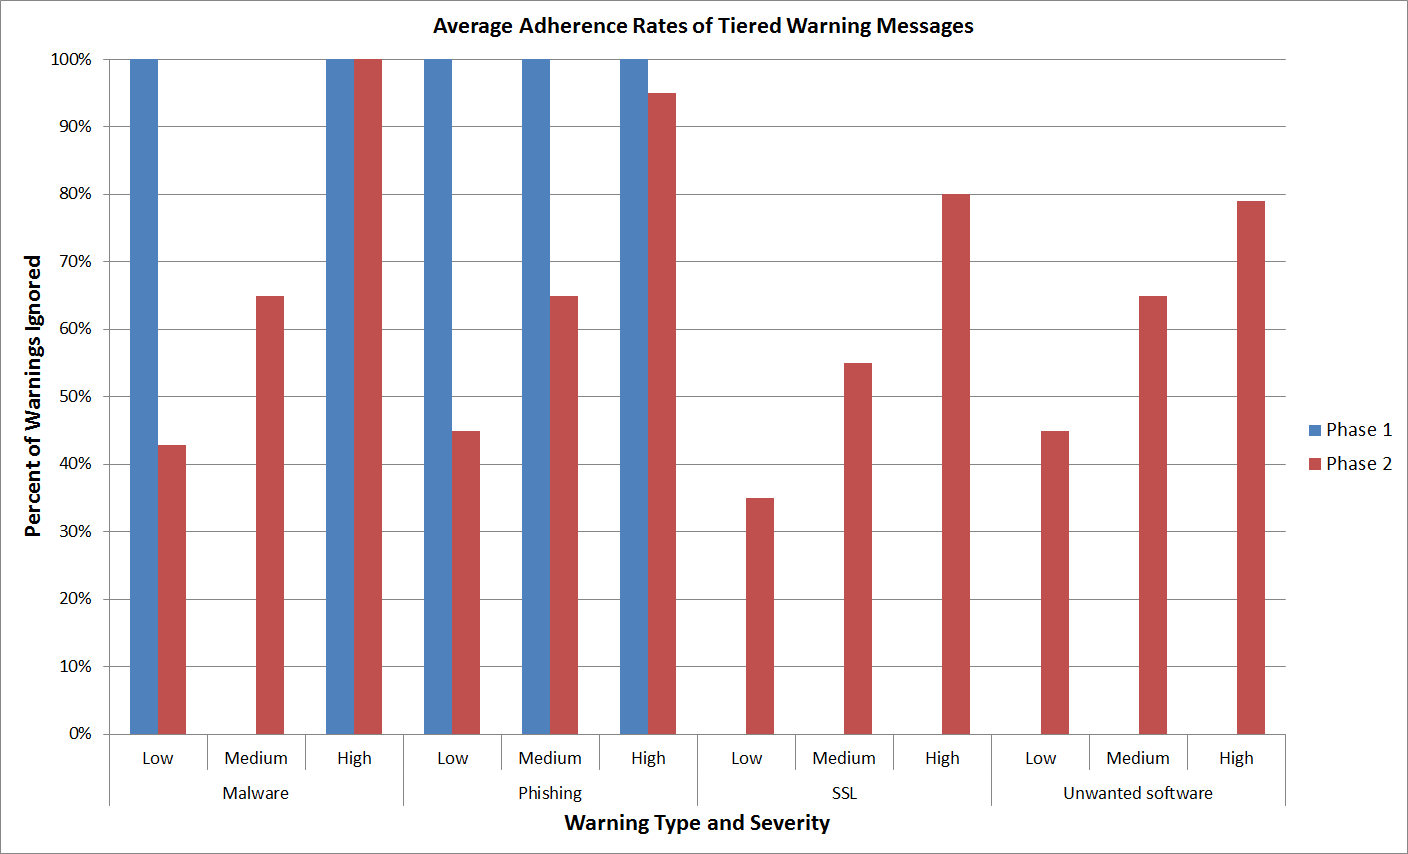
\includegraphics[width=\textwidth]{Figures/Adherence-Tiered}
	\decoRule
	\caption{User severity ratings for tiered warning messages}
	\label{fig:Severity-Tiered}
\end{figure}

\subsection{Severity Rating Analysis}
Six separate two-tailed t-tests were conducted. For each of the study phases, the mean user severity rating for the control warning messages was separately compared against the mean severity ratings for the low, medium, and high severity tiered messages.

In the first phase of the study, the mean user severity rating of the control messages was higher than the ratings of the low and high severity tiered warnings. However, this difference was not found to be statistically significant.

In the second phase of the study, the mean user severity rating was lower for the low and medium severity tiered messages when compared to the control messages (0.97 and 1.80, respectively, versus 2.70). In both cases, the difference was found to be statistically significant ($t(19) = 10.02, p = 5.09 \times 10^{-9}$ in the low severity versus control case and $t(19) = 6.03, p = 8.35 \times 10^{-6}$ in the medium severity versus control case). 

The mean user severity rating of the high severity tiered warnings in phase 2 was greater than that of the control warnings (3.30 versus 2.70). This difference was found to be statistically significant ($t(19) = -4.85, p = 0.0001$).

In summary, in phase 2, our ``severe'' tiered messages were rated as significantly more severe than the control messages by participants while our ``low'' and ``medium'' tiered messages were rated as significantly less severe than the control messages. This is consistent with the adherence rate findings in section \ref{Warning Adherence}.
